\documentclass[12pt]{article}
\usepackage{polski}
\usepackage[utf8]{inputenc}
\usepackage{graphicx}
\usepackage{amsmath}
\usepackage{graphicx}
\usepackage{setspace}
\usepackage{pdfpages}
\usepackage[T1]{fontenc}
\onehalfspacing

\title{ Wyznaczanie szerokości przerwy energetycznej
    półprzewodnika metodą termiczną (termistor) \\
    \large Informatyka – profil praktyczny, semestr II \\
    Wydział Matematyki Stosowanej \\
    Politechnika Śląska \\}

\author{ Sekcja 5 \\
    Piotr Skowroński, Bartłomiej Pacia}
\date{Maj 2022}

\begin{document}

\maketitle

\section{Wstęp teoretyczny}
Półprzewodnikami nazywamy substancje, na których konduktywność
można wpływać przez różne czynniki (najczęściej przez domieszkowanie
lub zmianę temperatury). Jest to spowodowane posiadaniem przerwy
energetycznej, ze specyficznego zakresu, między pasmem walencyjnym
a przewodnictwa (gdzie w przewodnikach ta przerwa jest jeszcze
mniejsza, a w izolatorach większa). Wyróżniamy następujące typy
półprzewodników:

Samoistne — posiadają niezanieczyszczoną sieć krystaliczną
(uporządkowane i symetryczne ułożenie atomów).

Domieszkowane – wprowadzenie do sieci krystalicznej elektronów
swobodnych innego atomu. W zależności różnicy liczby elektronów
domieszki od liczby elektronów półprzewodnika, domieszkowania
dzielimy na:

\indent \indent Typ p – pobieranie elektronu z półprzewodnika i
powstanie tzw. dziur elektronowych (naładowanie dodatnie).

\indent \indent Typ n – pobieranie elektronu z domieszki ułatwiając
przechodzenie w stan swobodny (naładowanie ujemne).

Teoria pasmowa ciał stałych — jest to teoria opisująca przewodnictwo
elektryczne. Pasmami energetycznymi nazywamy przedziały energetyczne,
jakie osiągają elektrony w danym atomie. Przerwą energetyczną,
nazywamy różnice energii między dwoma pasmami energetycznymi.
W elektronice najbardziej istotne są dwa pasma:

\indent \indent Walencyjne — przedział energetyczny elektronów
walencyjnych.

\indent \indent Przewodnictwa — przedział energetyczny elektronów
swobodnych, które stają się nośnikami prądu elektrycznego.

\section{Pomiary}

Podczas wykonywania doświadczenia w pracowni pomiary zapisywaliśmy ręcznie na
kartce. Następnie przepisaliśmy wyniki naszych pomiarów do pliku CSV, by
umożliwić ich wykorzystanie w programie.

Użyliśmy języka Python w środowisku Jupyter Notebook. Wykorzystaliśmy biblioteki
\textit{numpy}, \textit{pandas} i \textit{matplotlib}.
\section{Obliczenia}

\subsection*{Wykres $T(R_1)$ i $T(R_2)$ dla ogrzewania i ocieplania}
$0.01$V - 1$^{\circ}C$ \\
Przyjmujemy niepewności dla użytych przez nas urządzeń: \\
\indent $u(U) = \frac{0.5\% \cdot U+1 \cdot 0.001}{\sqrt{3}}$ \\
\indent $u(R_1) = \frac{1.5\% \cdot R_1 + 3 \cdot 0.01}{\sqrt{3}}$ \\
\indent $u(R_2) = \frac{0.8\% \cdot R_2 + 1 \cdot 0.01}{\sqrt{3}}$ \\
Tabelka z danymi. Lp. 1-11 ocieplanie, 12-22 ochładzanie:
\begin{center}
    \begin{tabular} { | c | c | c | c | c | c | c | }
        \hline
        Lp. & $U$, V & $u(U)$, V & $R_1$, k$\Omega$ & $R_2$, k$\Omega$ & $u(R_1)$, k$\Omega$ & $u(R_2)$, k$\Omega$ \\
        \hline
        1.  & 0.3080 & 0.0015    & 15.30            & 23.40            & 0.15                & 0.11                \\ \hline
        2.  & 0.3350 & 0.0015    & 13.40            & 20.50            & 0.13                & 0.10                \\ \hline
        3.  & 0.3600 & 0.0016    & 11.40            & 17.300           & 0.12                & 0.086               \\ \hline
        4.  & 0.3930 & 0.0017    & 10.20            & 15.700           & 0.11                & 0.078               \\ \hline
        5.  & 0.4250 & 0.0018    & 8.990            & 13.700           & 0.095               & 0.068               \\ \hline
        6.  & 0.4520 & 0.0019    & 7.410            & 11.400           & 0.081               & 0.058               \\ \hline
        7.  & 0.4780 & 0.0020    & 6.950            & 10.700           & 0.078               & 0.055               \\ \hline
        8.  & 0.5100 & 0.0020    & 6.010            & 9.400            & 0.069               & 0.049               \\ \hline
        9.  & 0.5370 & 0.0021    & 5.410            & 8.400            & 0.064               & 0.045               \\ \hline
        10. & 0.5790 & 0.0022    & 4.660            & 7.200            & 0.058               & 0.039               \\ \hline
        11. & 0.6010 & 0.0023    & 4.460            & 7.000            & 0.056               & 0.038               \\ \hline
        12. & 0.6010 & 0.0023    & 4.460            & 7.000            & 0.056               & 0.038               \\ \hline
        13. & 0.5780 & 0.0022    & 4.600            & 8.000            & 0.057               & 0.043               \\ \hline
        14. & 0.5340 & 0.0021    & 5.800            & 9.200            & 0.068               & 0.048               \\ \hline
        15. & 0.5120 & 0.0021    & 6.250            & 9.700            & 0.071               & 0.051               \\ \hline
        16. & 0.4690 & 0.0019    & 7.070            & 11.500           & 0.079               & 0.059               \\ \hline
        17. & 0.4500 & 0.0019    & 7.520            & 12.200           & 0.082               & 0.062               \\ \hline
        18. & 0.4260 & 0.0018    & 9.250            & 14.500           & 0.097               & 0.073               \\ \hline
        19. & 0.3920 & 0.0017    & 10.35            & 16.200           & 0.11                & 0.081               \\ \hline
        20. & 0.3680 & 0.0016    & 11.80            & 19.200           & 0.12                & 0.094               \\ \hline
        21. & 0.3370 & 0.0016    & 14.20            & 21.60            & 0.14                & 0.11                \\ \hline
        22. & 0.3120 & 0.0015    & 15.80            & 24.60            & 0.15                & 0.12                \\

        \hline
    \end{tabular}
\end{center}

Wykresy na następnych stronach
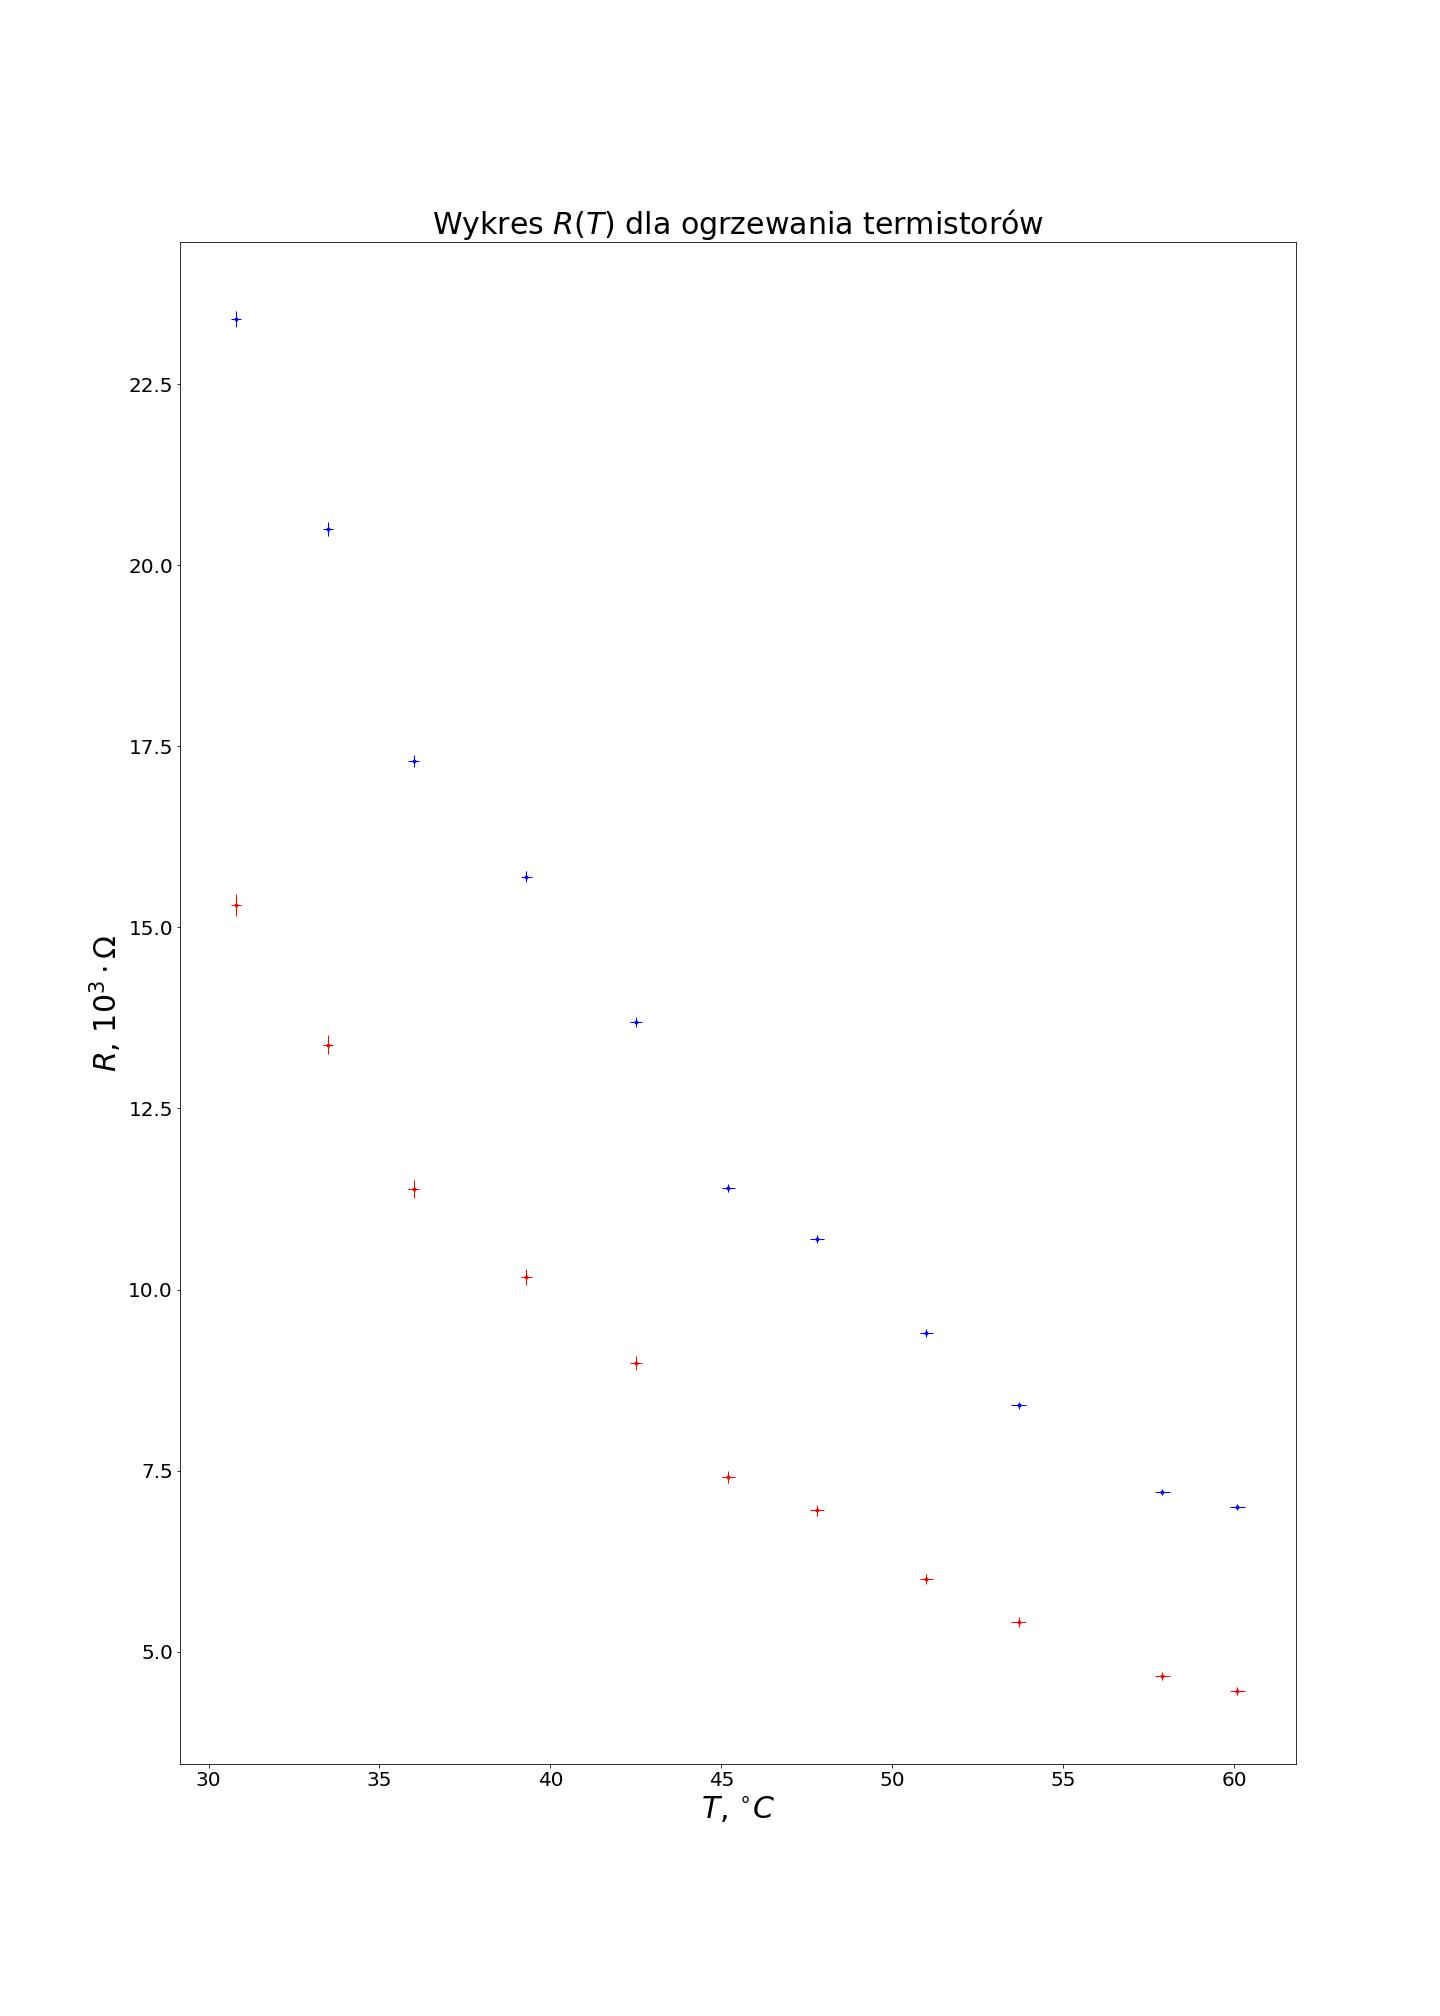
\includepdf{./img/wykres1.jpg}
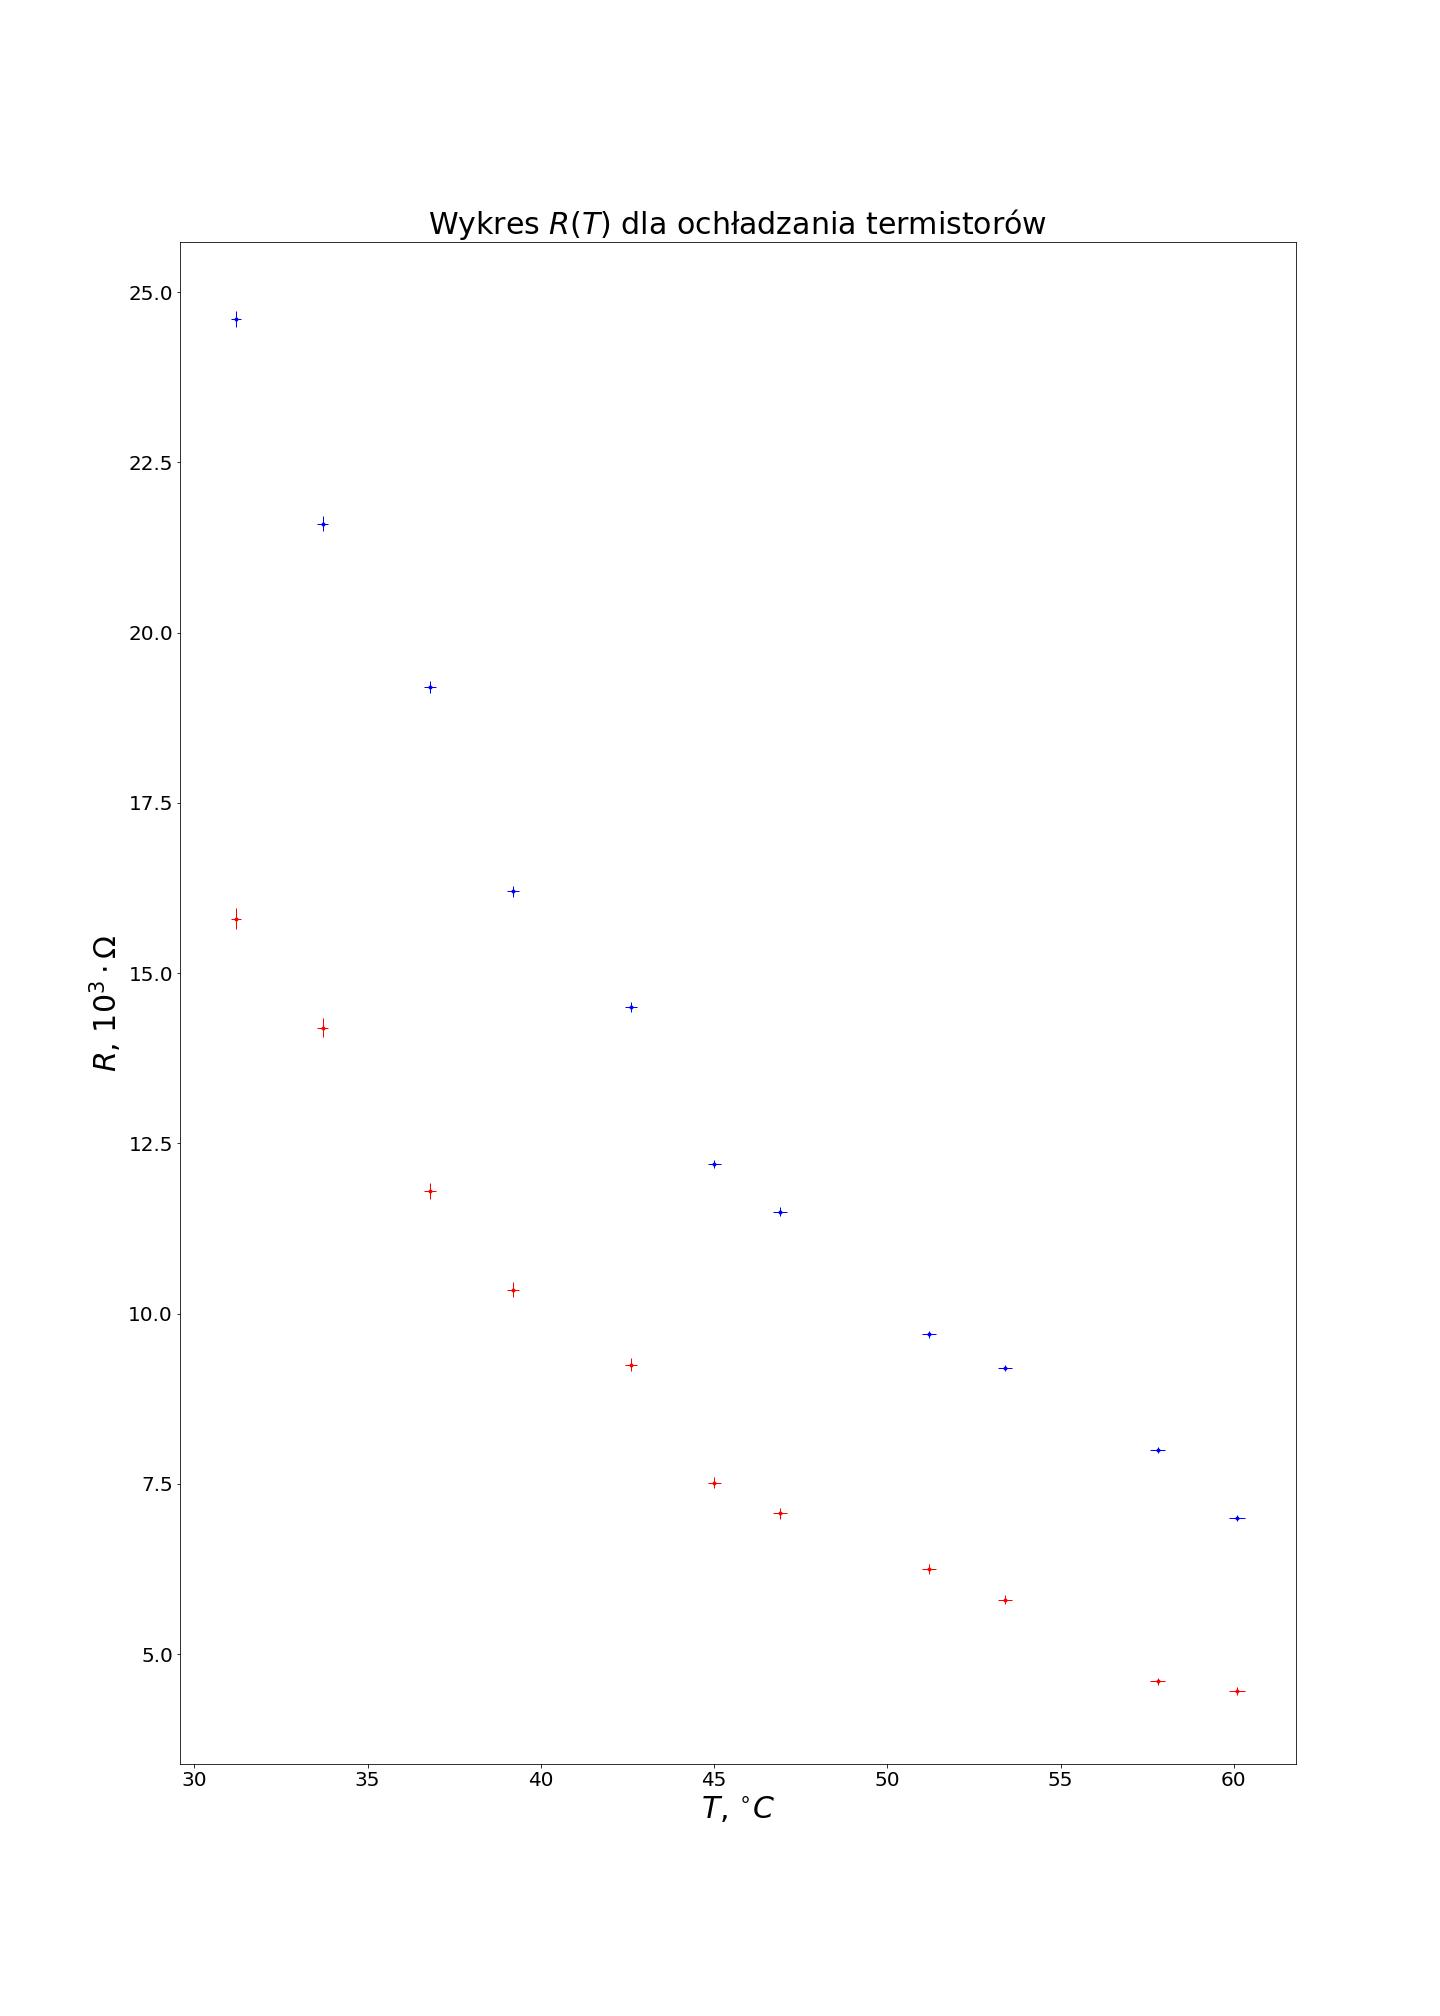
\includepdf{./img/wykres2.jpg}

\subsection*{Wykres $f(\frac{1}{T}) = \ln(R)$ dla ocieplania i ochładzania
    i \\ regresja liniowa}
Niepewności z prawa przenoszenia niepewności: \\
\indent $u(\frac{1}{T}) = \frac{u(T)}{T^2}$, $u(\ln(R)) = \frac{u(R)}{R}$. \\
Aby policzyć współczynniki kierunkowe prostych i wyrazy wolne skorzystamy ze
wzorów:
\begin{flushleft}

    \begin{center}
        $a = \frac{nS_{xy} - S_xS_y}{nS_{xx}-S_x^2}$, $b
            =\frac{S_{xx}S_y-S_xS_{xy}}{nS_{xx}-S_x^2}$
    \end{center}
    Gdzie: \\
    \begin{center}
        $S_x=\displaystyle\sum_{i=1}^{n}x_i$,
        $S_y=\displaystyle\sum_{i=1}^{n}y_i$,
        $S_{xx}=\displaystyle\sum_{i=1}^{n}x_i^2$,
        $S_{xy}=\displaystyle\sum_{i=1}^{n}x_i \cdot y_i$ \\
    \end{center}
\end{flushleft}

\begin{flushleft}
    Do obliczenia niepewności skorzystamy ze wzorów:
    \begin{center}
        $u(a) = \sqrt{\frac{n}{n-2} \cdot
                \frac{S_{\epsilon\epsilon}}{nS_{xx}-S_x^2}}$, $u(b) =
            \sqrt{\frac{1}{n-2} \cdot
            \frac{S_{xx}S_{\epsilon\epsilon}}{nS_{xx}-S_x^2}}$ \\
    \end{center}
    Gdzie: \\
    \begin{center}
        $S_{\epsilon\epsilon}=\displaystyle\sum_{i=1}^{n}\epsilon_i^2$, dla
        $\epsilon_i = y_i - ax_i - b$
    \end{center}

\end{flushleft}
Współczynniki dla ocieplania termistorów:

$a_1 = 4330$ K, $a_2 = 4250$ K,

$b_1 = -11.5$, $b_2 = -10.8$. \\
Niepewności współczynników:

$u(a_1) = 180$ K, $u(a_2) = 240$ K,

$u(b_1) = 0.57$, $u(b_2) = 0.74$. \\
Postać końcowa współczynników:

$a_1 = 4330(180)$ K, $a_2 = 4250(240)$ K,

$b_1 = -11.50(57)$, $b_2 = -10.80(74)$. \\
Współczynniki dla ochładzania termistorów:

$a_1 = 4420$ K, $ a_2 = 4260$ K,

$b_1 = -11.8$, $b_2 = -10.8$. \\
Niepewności współczynników:

$u(a_1) = 110$ K, $u(a_2) = 140$ K,

$u(b_1) = 0.34$, $u(b_2) = 0.43$. \\
Postać końcowa współczynników:

$a_1 = 4420(110)$ K, $a_2 = 4260(140)$ K,

$b_1 = -11.80(34)$, $b_2 = -10.80(43)$. \\
Wykresy na następnych stronach:

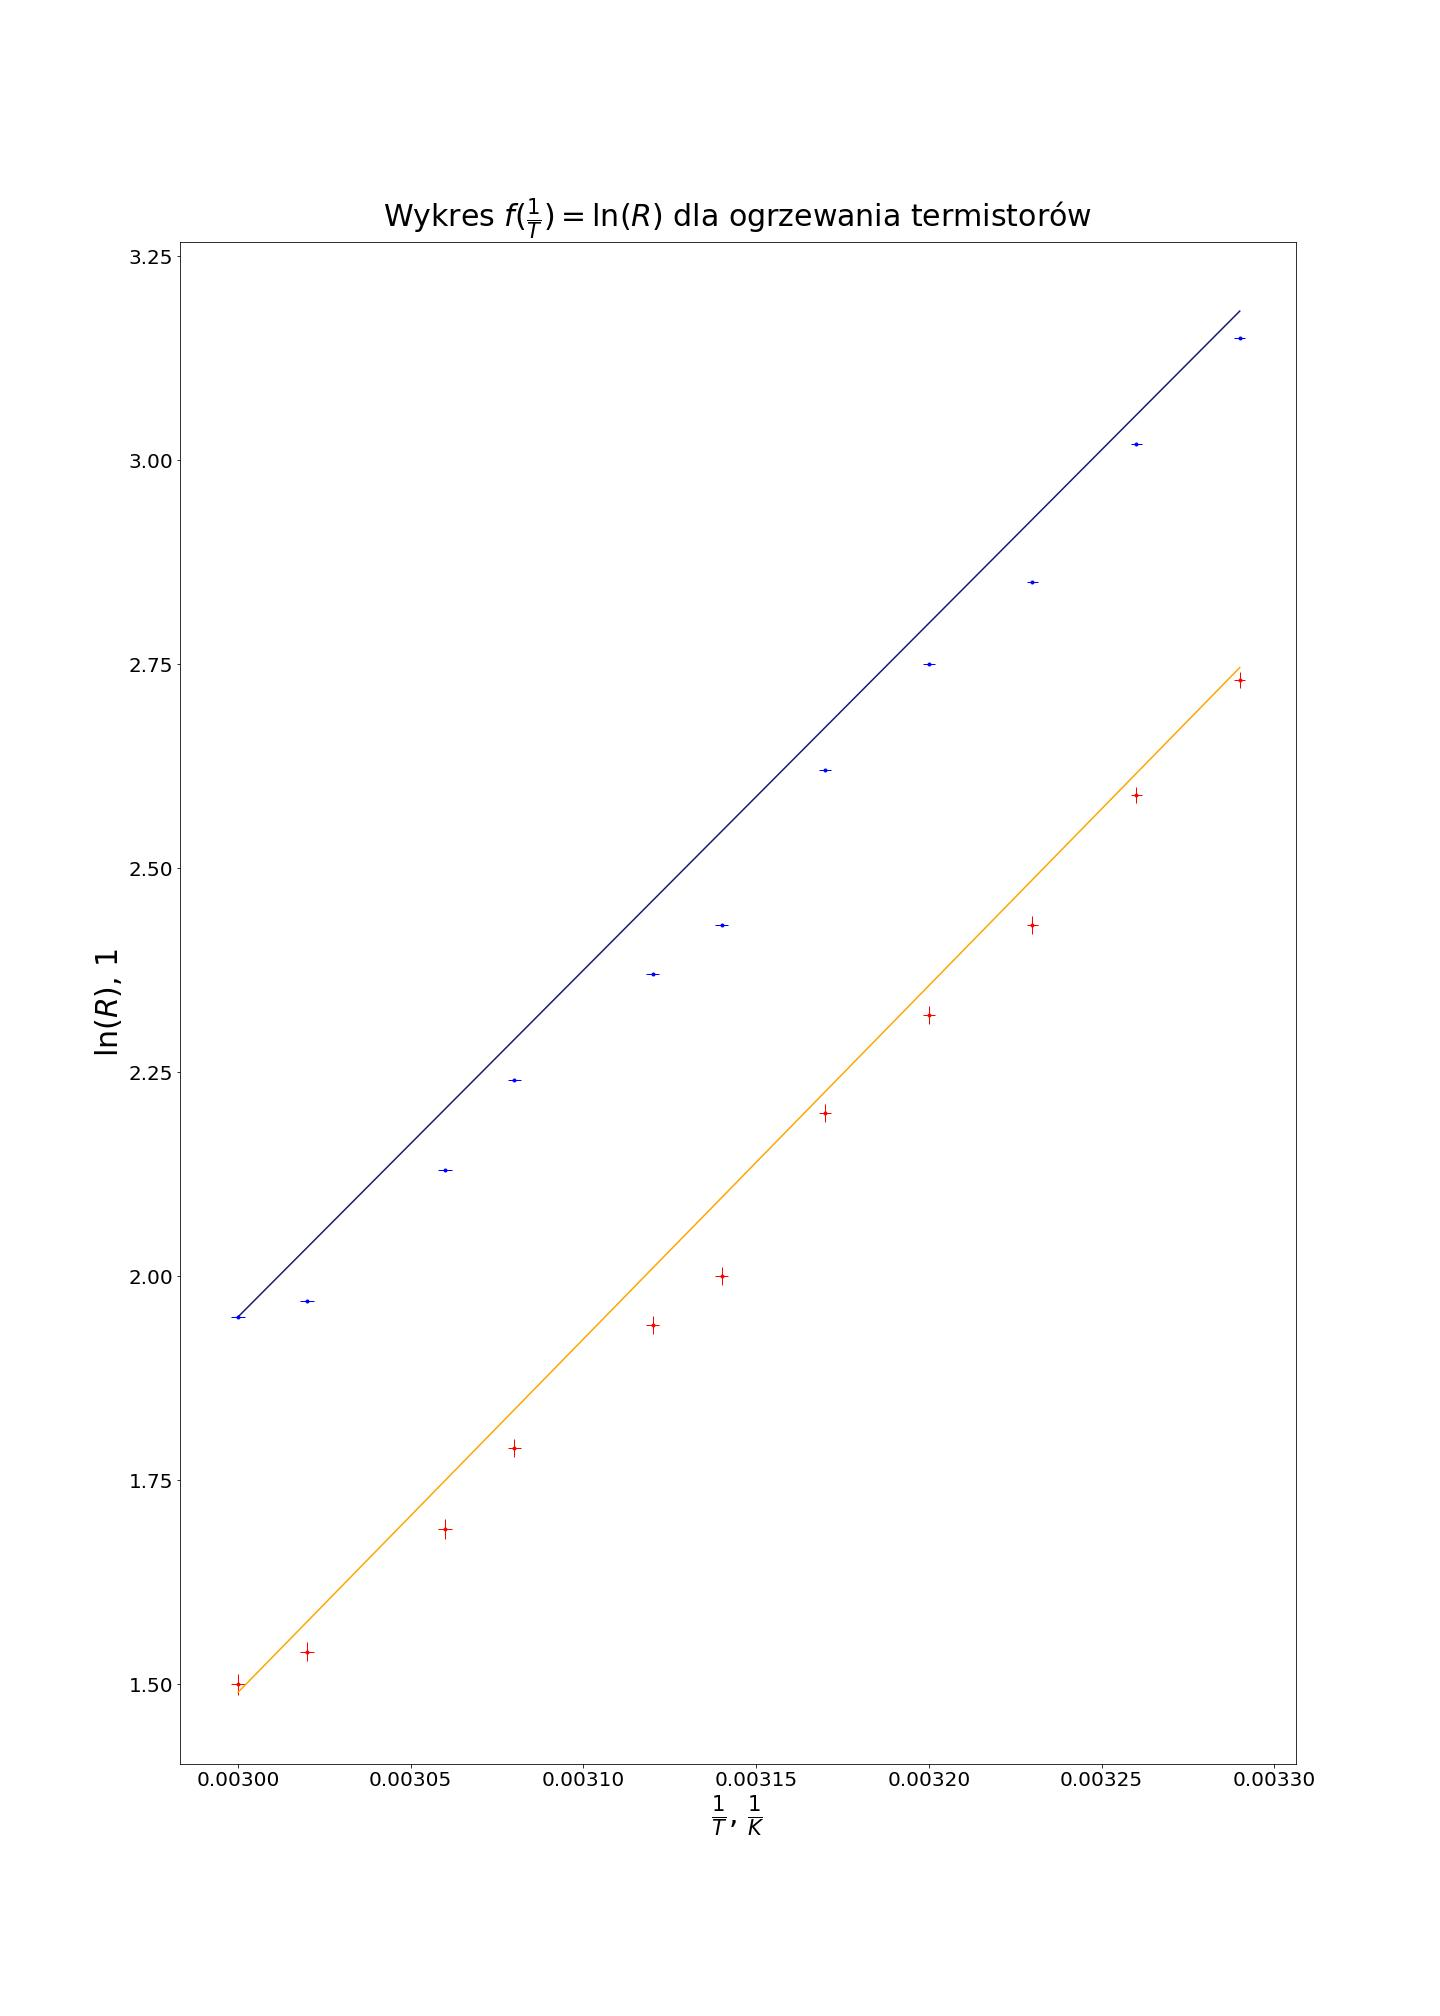
\includepdf{./img/wykres3.jpg}
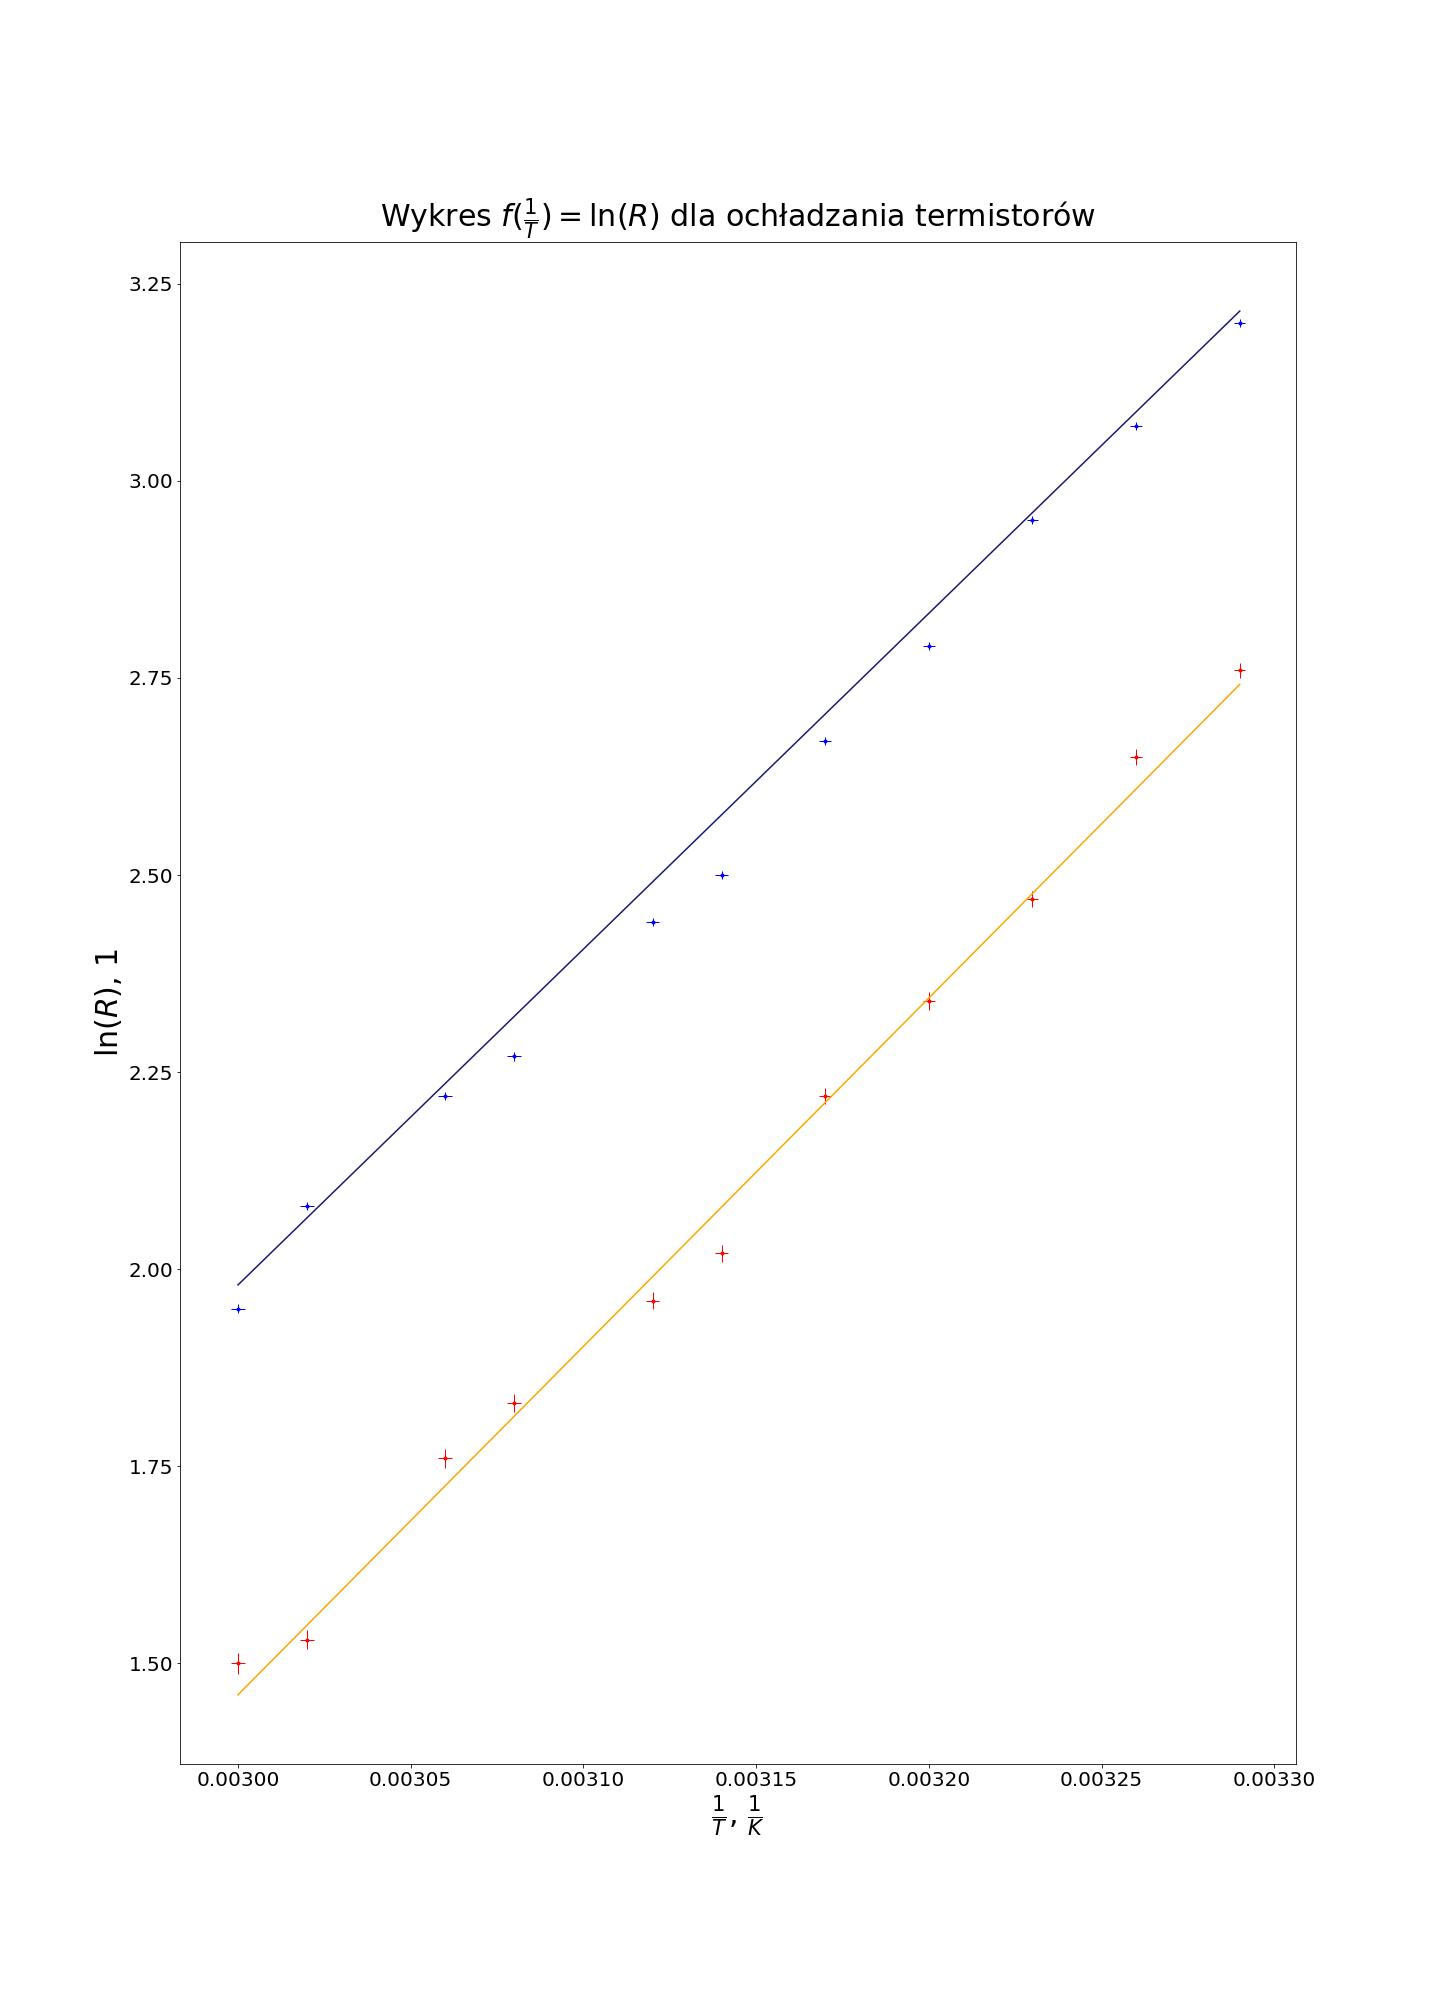
\includepdf{./img/wykres4.jpg}

\subsection*{Wyznaczenie szerokości przerw energetycznych $\Delta E$
    dla obu termistorów}
Ze wzoru $\ln(R) = \frac{\Delta E}{2k} \cdot \frac{1}{T} + \ln{R_0}$
wyznaczamy współczynnik kierunkowy $a = \frac{\Delta E}{2k}$ \\
Zatem wzór na szerokość przerwy energetycznej ma postać:
\begin{center} $\Delta E = 2ka$ \end{center}
$1$J = $6.24 \cdot 10^{18}$eV \\
Podczas ocieplania termistorów: \\
\indent $\Delta E_1 = 0.747$ eV,\\
\indent $\Delta E_2 = 0.733$ eV. \\
Podczas chłodzenia termistorów: \\
\indent $\Delta E_1 = 0.762$ eV, \\
\indent $\Delta E_2 = 0.734$ eV.

\subsection*{Obliczenie niepewności szerokości przerwy energetycznej
    $u(\Delta E)$ korzystając z prawa przenoszenia niepewności}


Niepewność $u(\Delta E)$ wyznaczamy z prawa przenoszenia niepewności:
\begin{center}
    $u(\Delta E) = 2k \cdot u(a)$.
\end{center}
Po obliczeniach dla ogrzewania termistorów:
\begin{center}
    $u(\Delta E_1) = 0.031$ eV, \\
    $u(\Delta E_2) = 0.041$ eV.
\end{center}
Po obliczeniach dla ochładzania termistorów:
\begin{center}
    $u(\Delta E_1) = 0.019$ eV, \\
    $u(\Delta E_2) = 0.024$ eV.
\end{center}

\subsection*{Zapisanie wyników w odpowiednim formacie}
Dla ogrzewania termistorów:
\begin{center}
    $\Delta E_1 = 0.747(31)$ eV, \\
    $\Delta E_2 = 0.733(41)$ eV.
\end{center}
Dla ochładzania termistorów:
\begin{center}
    $\Delta E_1 = 0.762(19)$ eV, \\
    $\Delta E_2 = 0.734(24)$ eV.
\end{center}

\subsection*{Test zgodności dla obu termistorów}
Liczymy niepewność rozszerzoną
\begin{center}
    $U(x_1 - x_2) = k\sqrt{[u(x_1)]^2+[u(x_2)]^2}$.
\end{center}
W miejsce $x$ i $u(x)$ wstawiamy $\Delta E$ i $u(\Delta E)$,
przyjmujemy $k = 2$
\begin{center}
    $U(\Delta E_1 - \Delta E_2) = 2\sqrt{[u(\Delta E_1)]^2+[u(\Delta E_2)]^2}$. \\
\end{center}
Niepewność rozszerzona dla ocieplania termistorów
\begin{center}
    $U(\Delta E_1 - \Delta E_2) = 0.10$ eV.
\end{center}
Niepewność rozszerzona dla ochładzania termistorów
\begin{center}
    $U(\Delta E_1 - \Delta E_2) = 0.061$ eV.
\end{center}
Wyniki pomiaru uważa się za zgodne jeśli
\begin{center}
    $|\Delta E_1 - \Delta E_2| < U(\Delta E_1 - \Delta E_2)$.
\end{center}
Dla naszych pomiarów
\begin{center}
    $0.014$ eV < $0.103$ eV, \\
    $0.028$ eV < $0.061$ eV.
\end{center}
Co pokazuje, że termistory są jednakowe.

\section{Wnioski}
Przy pomocy tego doświadczenia udało się wyznaczyć
szerokości przerw energetycznej dla obu termistorów. Z wykresów
widać, że wraz ze wzrostem temperatury opór maleje, co jest zgodne
ze wzorem teoretycznym. Dodatkowo otrzymane szerokości przerw
energetycznych dla obu termistorów spełniają test zgodności, co
oznacza, że zostały one wykonane z tych samych materiałów.
\end{document}